% ******************************************************** %
%              TEMPLATE DE INFORME ORGA2 v0.1              %
% ******************************************************** %
% ******************************************************** %
%                                                          %
% ALGUNOS PAQUETES REQUERIDOS (EN UBUNTU):                 %
% ========================================
%                                                          %
% texlive-latex-base                                       %
% texlive-latex-recommended                                %
% texlive-fonts-recommended                                %
% texlive-latex-extra?                                     %
% texlive-lang-spanish (en ubuntu 13.10)                   %
% ******************************************************** %


\documentclass[a4paper]{article}
\usepackage[utf8]{inputenc}
\usepackage{charter}   % tipografia
\usepackage{graphicx}
%\usepackage{makeidx}
\usepackage{paralist} %itemize inline

\usepackage{float}
\usepackage{mathtools}
%\usepackage{amsmath, amsthm, amssymb}
%\usepackage{amsfonts}
%\usepackage{sectsty}
%\usepackage{charter}
\usepackage{wrapfig}
%\usepackage{listings}
%\lstset{language=C}
\usepackage{tikz}
\usetikzlibrary{patterns,arrows,decorations.pathmorphing,backgrounds,positioning,fit,petri,decorations.pathreplacing}
\usepackage{bytefield}
\usepackage[english,spanish]{babel}
% \setcounter{secnumdepth}{2}
\usepackage{underscore}
\usepackage{caratula}
\usepackage{url}
\usepackage{hyperref}
\usepackage{graphicx}
\usepackage{amsmath}
\usepackage{algorithm}
\usepackage{algpseudocode}
\usepackage{titlesec}
\usepackage{tikz}
\usepackage{subcaption}

\usetikzlibrary{arrows}

\DeclarePairedDelimiterX{\norm}[1]{\lVert}{\rVert}{#1}

% https://tex.stackexchange.com/questions/60209/how-to-add-an-extra-level-of-sections-with-headings-below-subsubsection
\setcounter{secnumdepth}{4}
\titleformat{\paragraph}
{\normalfont\normalsize\bfseries}{\theparagraph}{1em}{}
\titlespacing*{\paragraph}
{0pt}{3.25ex plus 1ex minus .2ex}{1.5ex plus .2ex}



\makeatletter
\def\BState{\State\hskip-\ALG@thistlm}
\makeatother

% ********************************************************* %
% ~~~~~~~~              Code snippets             ~~~~~~~~~ %
% ********************************************************* %

\usepackage{color} % para snipets de codigo coloreados
\usepackage{fancybox}  % para el sbox de los snipets de codigo

\definecolor{litegrey}{gray}{0.94}

\newenvironment{codesnippet}{%
	\begin{Sbox}\begin{minipage}{\textwidth}\sffamily\small}%
	{\end{minipage}\end{Sbox}%
		\begin{center}%
		\vspace{-0.4cm}\colorbox{litegrey}{\TheSbox}\end{center}\vspace{0.3cm}}



% ********************************************************* %
% ~~~~~~~~         Formato de las páginas         ~~~~~~~~~ %
% ********************************************************* %

\usepackage{fancyhdr}
\pagestyle{fancy}

%\renewcommand{\chaptermark}[1]{\markboth{#1}{}}
\renewcommand{\sectionmark}[1]{\markright{\thesection\ - #1}}

\fancyhf{}

\fancyhead[LO]{Sección \rightmark} % \thesection\ 
\fancyfoot[RO]{\thepage}
\renewcommand{\headrulewidth}{0.5pt}
\renewcommand{\footrulewidth}{0.5pt}
\setlength{\hoffset}{-0.8in}
\setlength{\textwidth}{16cm}
%\setlength{\hoffset}{-1.1cm}
%\setlength{\textwidth}{16cm}
\setlength{\headsep}{0.5cm}
\setlength{\textheight}{25cm}
\setlength{\voffset}{-0.7in}
\setlength{\headwidth}{\textwidth}
\setlength{\headheight}{13.1pt}

\renewcommand{\baselinestretch}{1.1}  % line spacing

% ******************************************************** %


\begin{document}


\thispagestyle{empty}
\materia{métodos Numericos}
\submateria{Primer Cuatrimestre de 2020}
\titulo{Trabajo Práctico 1}
\subtitulo{Sistemas de ecuaciones lineales}
\integrante{Manuel Panichelli}{72/18}{panicmanu@gmail.com}
\integrante{Tomas Tropea}{115/18}{tomastropeaa@gmail.com}
\integrante{Ignacio Alonso Rehor}{195/18}{arehor.ignacio@gmail.com}

\maketitle
\newpage

\thispagestyle{empty}
\vspace{3cm}
\setcounter{tocdepth}{4}
\setcounter{secnumdepth}{5}
\tableofcontents

\section{Abstract}

Se aborda la problemática de la confección de rankings para competencias deportivas. Se comparan los métodos CMM y WP y sus posibles problemas. Finalmente se realiza una comparación de diferentes heurísticas para tener el mayor ranking posible, con la menor cantidad de victorias.

Se concluye que el método CMM es superior a WP, que es justo, y que refleja la habilidad real de los equipos involucrados.

\textit{\textbf{keywords} colley matrix method, winning percentage, rankings simulados, errores de calculo}

\section{Introducción}

Las competencias deportivas presentan una problemática compleja al momento de intentar clasificar a los distintos competidores por su desempeño. Este problema es inevitable, ya que el deporte demanda tener una forma de establecer un ranking entre los involucrados en el mismo. 

Los distintos métodos que intentan abordar este problema utilizan estrategias variadas. Hay metodos que involucran el porcentaje de victorias de un equipo, o tienen en cuenta contra quienes se enfrentó el equipo para poder ponderar mas sus victorias contra buenos equipos y sus derrotas contra malos equipos. Es importante notar que, a veces son suficientes para lograr resultados reales métodos simples como el porcentaje de victorias. Este es el caso de las competencias donde los competidores juegan todos contra todos, ya que utilizar este criterio parece ser suficiente para clasificarlos.

Estas ideas, aunque sean realistas para ciertos casos, no siempre funcionan en la practica. Esto se debe a que no capturan toda la información que hubo durante una serie de partidos, como que oponentes se enfrentaron, cuantos partidos hubo entre ellos, etc. Es valido preguntarse si realmente suceden estas cosas, pero hay ejemplos concretos como el de ATP, donde no se juegan la misma cantidad de juegos entre competidores, que presenta este problema.

Para sumarle otro problema a esto, los rankings producidos pueden, en ciertos casos, determinar entre uno y otro equipo que pase una clasificación importante. Esto resulta en que el ranking resultante no sea una cuestión menor, sino que puede determinar cuestiones económicas importantes para un equipo, así también como merito deportivo.

Debido a estas razones nos proponemos investigar y estudiar dos métodos, con el objetivo de poder determinar la eficacia de cada uno en distintos contextos, y como implementaciones diferentes de ellos pueden variar el ranking, y en que se diferencian a la hora de determinarlo.

El metodo \textbf{WP (Winning Percentage)} es una forma simple de calcular el ranking de un conjunto de equipos. Propone una formula que resulta natural para definir el rating de un equipo basado en los resultados de sus partidos. Define $r_{i}$, el rating del i-esimo equipo como:

\begin{align*}
    r_{i} &= (\frac{w_{i}}{w_{i}+l_{i}})
\end{align*}

Donde $w_{i}$ son los partidos ganados y $l_{i}$ son los partidos perdidos por el i-esimo equipo.
Dado este metodo, podemos plantear un sistema de n ecuaciones equivalente a:

\begin{align*}
    r_{1} &= (\frac{w_{1}}{w_{1}+l_{1}})\\
    r_{2} &= (\frac{w_{2}}{w_{2}+l_{2}})\\
    & \vdots \\
    r_{n} &= (\frac{w_{n}}{w_{n}+l_{n}})
\end{align*}

Notar que cada ecuación presenta una sola incógnita, $r_{i}$, ya que los partidos ganados $w_{i}$ y perdidos $l_{i}$ son conocidos para cada equipo. Esto implica que no es necesario plantear un sistema matricial para resolver el sistema, sino que puede resolverse cada ecuación individualmente, haciendo que este método sea muy sencillo de calcular.

Por otro lado, el \textbf{Colley Matrix Method (CMM)} es una versión mas avanzada del método WP mencionado anteriormente. Busca determinar el rating de cada uno de los equipos a partir de sus partidos, planteando un sistema de ecuaciones lineales, y resolviendo el sistema:

\begin{align*}
Cr = b
\end{align*}

Siendo $r$ el vector de ratings de cada equipo, $b$ el vector de longitud igual a la cantidad de equipos, siendo el i-esimo coeficiente correspondiente al i-esimo equipo, equivalente a la expresion:

\begin{align*}
b_{i} &= 1 + \frac{w_{i}-l{i}}{2}
\end{align*}

Donde $w_{i}$ son los partidos ganados y $l_{i}$ los perdidos por el i-esimo equipo.

Por otro lado, $C$ es \textit{la matriz de Colley} definida de la siguiente manera:

\[ C_{ij}=
    \begin{cases} 
      -n_{ij} & i\neq j \\
      2+n_{i} & i=j
   \end{cases}
\]

Es decir, el elemento $c_{ij}$, donde $i \neq j$, es la cantidad de partidos del equipo $i$ contra el oponente $j$ con signo negativo.

\section{Desarrollo}

\subsection{Implementaciónes de Métodos Numericos}

Para poder evaluar los distintos aspectos de los metodos de CMM y WP, y poder llevar a cabo experimentaciones de los mismos, vamos a necesitar tener implementaciones de los mismos. Por esta razon, decidimos implementar una version de cada metodo en C++. Por un lado, tenemos una version iterativa del metodo WP, y por otro una  version que resuelve el sistema planteado por CMM. Hablaremos primero entonces de estas implementaciones y los distintos detalles y consideraciones que tuvimos en cuenta para realizarlos.

\subsubsection{Algoritmo WP}

El metodo de WP plantea una ecuación para el rating de cada equipo, con una sola incógnita, permitiendo un algoritmo simple para resolverlas. El siguiente pseudocódigo lo ilustra:

\begin{algorithm}
\caption{WP}\label{wp}
\begin{algorithmic}[1]
\Procedure{WP}{\textrm{games: List[Game]}}
\State $\textit{ratings} \gets \textit{vector of size N}$
\For{\texttt{i = 1 to N}}
    \State wins $\gets$ 0
    \State total $\gets$ 0
	\For{\texttt{j = 1 to games.size}}
	    \If{games[j].team1 == i \textbf{or} games[j].team2 == i}
	        \State total $\gets$ total +1
	        \If{games[i].win == i}
	            \State wins $\gets$ wins + 1
\State\textbf{end for}
    
	\State ratings[i] $\gets$ wins/total

\State\textbf{end for}
\State \textbf{return} $\textit{ratings}$
\EndProcedure
\end{algorithmic}
\end{algorithm}

\subsubsection{CMM}

\paragraph{Características de Matriz de Colley}

Si recordamos la definición de la matriz de Colley, es evidente que la suma de los módulos de los elementos de la fila $i$, excluyendo la diagonal, nos da como resultado la cantidad de partidos totales que jugo el equipo $i$, es decir $n_{i}$ que es estrictamente menor que $n_{i} + 2$, que es precisamente la definición del elemento en la diagonal de la fila $i$, es decir $c_{ii}$. Esto nos dice que la matriz de Colley resulta una matriz \emph{estrictamente diagonal dominante}.

A partir de esta caracterización de la matriz de Colley podemos ver que se cumplen varias propiedades interesantes. La primera siendo que todas sus submatrices principales también son matrices estrictamente diagonal dominantes, lo que nos dice que estas submatrices principales, son inversibles. Entonces, como todas las submatrices principales de la matriz de Colley son inversibles, podemos garantizar que existe una factorización particular de la matriz de Colley llamada \emph{factorización LU}.

La existencia de esta factorización para la matriz de Colley, nos indica que se puede triangular mediante el método de eliminación de Gauss, sin necesidad de hacer permutaciones entre filas. Es por esta razón que en este caso particular no es necesario hacer pivoteo parcial en la implementación de eliminación gausseana.

Una última propiedad que resulta útil de la matriz de Colley es la de su simetría. Como el elemento en la posición $i,j$, donde $i \neq j$, representa la cantidad de partidos del equipo $i$ contra el oponente $j$, con signo negativo, entonces, el elemento en la posición $j,i$ debería representar la cantidad de partidos del equipo $j$ contra el oponente $i$, con signo negativo, que lógicamente deben ser iguales. O lo que es igual $c_{ij} = c_{ji}$, que es la definición de una matriz simétrica.

\paragraph{Eliminación Gausseana para CMM}

A continuación tenemos el algoritmo que hace la eliminación gausseana sobre el sistema $Cr = b$, siendo $C$ y $b$ la matriz y el vector generados por el método de Colley:

\begin{algorithm}
\caption{Gaussian Elimination}\label{euclid}
\begin{algorithmic}[1]

\Procedure{Gaussian Elimination}{$system$}

\State $\textit{A} \gets \textit{system.A}$
\State $\textit{b} \gets \textit{system.b}$

\For{\texttt{i = 0 to matrix.rows-1}}
    \For{\texttt{j = i+1 to matrix.rows-1}}
        \State $\textit{coeff} \gets \textit{A.cells[i][j]/A.cells[i][i]}$
        \For{\texttt{c = 0 to matrix.cols-1}}
            \State $\textit{A.cells[j][c]} \gets \textit{A.cells[j][c] - A.cells[i][c]*coeff}$
        \EndFor
		\State $\textit{b[j]} \gets \textit{b[j] - b[i]*coeff}$
    \EndFor
\EndFor

\State \textbf{return} $\textit{system}$
\EndProcedure
\end{algorithmic}
\end{algorithm}

Tenemos inicialmente el sistema a resolver, con la matriz A y el vector b. Luego, iteramos cada fila de la matriz, siendo m el numero de la fila. En cada paso, tomamos la fila numero m en la que estamos parados y le restamos a cada una de las filas por abajo de esta un multiplo k de ella. En la linea 6 se puede ver como se calcula este coeficiente k. Si tenemos la fila numero n, y queremos restarle un multiplo de la fila m, para poner un 0 en la posicion n de la fila m, tenemos que calcular como muestra la linea 6:

\begin{align*}
k &= a_{nm} - a_{mm}
\end{align*}

Es decir, el coeficiente en la posición m de la fila n a la que queremos restarle, dividido el coeficiente en la diagonal que se corresponde a la fila n que vamos a usar para restar. Luego tomamos este coeficiente y hacemos lo que muestran la linea 7 y 8:

\begin{align*}
f_{n} &= f_{n} - k* f_{m}
\end{align*}

Esto pone efectivamente un 0 en la posicion m de la fila n, ya que la resta queda:
\begin{align*}
a_{nm} &= a_{nm} - a{nm}\cdot(\frac{a_{nm}}{a_{mm}})\\
&= a_{nm} - a_{nm}\cdot(\frac{a_{mm}}{a_{mm}})\\
&= a_{nm} - a_{nm}\cdot1 = 0
\end{align*}

también se le resta al coeficiente b que se corresponde con la fila n con el mismo calculo, como se ve en la linea 10: 
\begin{align*}
b_{n} = b_{n} - k * b_{m}
\end{align*}

Por la forma en que se recorre la matriz, este algoritmo genera una matriz triangular superior. Resta aplicar el metodo de backward substitution, como se muestra a continuacion:

\begin{algorithm}
\caption{Backward substitution}\label{bs}
\begin{algorithmic}[1]

\Procedure{Backward substitution}{$system$}

\State $\textit{A} \gets \textit{system.A}$
\State $\textit{b} \gets \textit{system.b}$
\State $\textit{x} \gets \textit{vector of size A.rows}$

\For{\texttt{r = A.rows-1 to 0}}
    \State $\textit{sum} \gets \textit{0}$
    \For{\texttt{c = r+1 to A.cols-1}}
        \State $\textit{sum} \gets \textit{sum + x[c]*A.cells[r][c]}$
    \EndFor
	\State $\textit{x[r]} \gets \textit{(b[r] - sum) / A.cells[r][r]}$
\EndFor
\State \textbf{return} $\textit{x}$
\EndProcedure
\end{algorithmic}
\end{algorithm}

En este paso lo que hacemos es empezar desde la ultima fila y subir hasta la primera, ya que la matriz es triangular superior. En cada paso utilizamos los ratings que ya despejamos de resolver ecuaciones anteriores, y hacemos la sumatoria de:
\begin{align*}
suma &= \sum_{c=r+1}^{n} a_{rc} * x_{c} 
\end{align*}

Donde c empieza en r+1 y va hasta columnas de A menos 1. Esto produce una sumatoria sin el elemento de la diagonal, porque es el que queremos averiguar. Finalmente tomamos esta sumatoria y despejamos el rating de la diagonal de esa fila, de la siguiente manera, como muestra la linea 10:

\begin{align*}
x_{r} &= \frac{(b_{r} - suma)}{a_{rr}}
\end{align*}

%\textcolor{red}{factorización LU ref/completar/} de la matriz, y lo que es más, se va a poder triangular mediante el método de eliminación de Gauss-Jordan sin necesidad de permutar entre filas. \textcolor{red}{completar}

%que las submatrices principales también lo son. Como las matrices diagonal dominantes son inversibles, esto implica que las submatrices principales de toda matriz diagonal dominante son inversibles, y esto último es una condición suficiente para que la matriz C admita una factorización LU, es decir, se puede triangular mediante el método de eliminación Gauss-Jordan sin necesidad de permutar entre filas ni columnas.

\paragraph{Estabilidad numerica}

Al realizar esta implementación, nos preguntamos los posibles problemas que podia tener la eliminación gausseana en terminos de establidad numerica por el uso de aritmetica finita. 

A diferencia de los numeros con los que trabajamos normalmente, que pueden tener infinitas cifras, en la computadora se pueden representar con finitas cifras, lo cual genera perdida de precisión. Esta perdida de precisión puede ser minima o no, dependiendo de que paso el los calculos intermedios para encontrar el resultado final. Podemos listar los casos que generan problemas dependiendo de la operación que se realiza:

\begin{itemize}
    \item Dividir por números pequeños.
    \item Multiplicar por numeros grandes.
    \item Restar numeros similares (Cancelacion catastrofica)
    \item Sumar numeros de magnitudes distintas.
\end{itemize}

En los primeros dos casos, se genera un error al momento del redondeo proporcional a los numeros que se utilizaron. En el tercer caso se produce una perdida de los digitos significativa y en el ultimo caso, el numero de menor magnitud puede llegar a no afectar a la suma.

Por estas razones es que, al momento de realizar la eliminacion gausseana, se debe tener cuidado con el aspecto de la division por numeros pequeños. Es por esta misma razon que se introduce la tecnica de pivoteo, donde se utiliza la fila que tenga el coeficiente mas grande en cada paso para dividir.

Debido a las caracteristicas de la matriz de Colley, esto no es necesario. Por ser diagonal dominante, el elemento de la diagonal es el mas grande en valor absoluto de la fila, y por ser simetrica, también de la columna. Como esta propiedad se mantiene luego de cada paso de eliminacion gausseana para la submatriz que falta triangular, garantiza que el pivoteo parcial nunca hará una permutacion. Entonces obtendremos una buena estabilidad numérica sin necesidad de agregar pivoteo al algoritmo descripto anteriormente.

\subsection{Error del método CMM}

Hemos mencionado anteriormente como, al realizar el método de eliminación de Gauss, pueden generarse errores debido al uso de aritmética finita. Por esta razón, quisimos realizar un experimento analizando el grado de error que podía presentar nuestra implementación. Así mismo, quisimos incluir en este análisis a los resultados brindados por la cátedra. Dado que no estamos comparando contra los resultados provistos por la cátedra, el lector podría preguntarse entonces, contra qué resultados es válida la comparación, pues, después de todo, estos también deberían estar sujetos a algún grado de error. La solución que se nos ocurrió fue, dada una muestra, armar el sistema asociado a la matriz de Colley, y resolverlo usando la biblioteca \texttt{numpy.linalg}\footnote{https://docs.scipy.org/doc/numpy/reference/generated/numpy.linalg.solve.html}. Por este motivo, vale aclarar que este experimento y sus resultados, no son totalmente determinantes, si no, más bien, sirven para darle al lector una idea del grado de error que admiten ambas implementaciones.
Con estos supuestos asumidos, la próxima pregunta que podría realizarse el lector es, cómo medir el grado de error que presenta una implementación contra nuestro sujeto de comparación, pues, después de todo, esta comparación debe hacerse entre dos vectores. Lo habitual en estos casos es calcular la distancia vectorial entre estos dos resultados, donde, dados $v,w$ en un espacio vectorial, y $\norm{\cdot}$ una norma del mismo espacio vectorial, se define:

\[d(v,w) = \norm{v-w}\]

Lo interesante de este enfoque es que nos permite analizar cómo afecta, la elección de distintas normas vectoriales, al resultado final. Para evaluar este punto, decidimos calcular las distancias considerando tres normas vectoriales usuales: la norma euclídea, la norma-1 , y por último la norma infinito.

\subsection{Comparativa entre métodos}

Dependiendo de la competencia con la que se trate, los datos de partidos pueden variar significativamente. El schedule puede ser tal que todos los equipos se enfrenten contra todos equitativamente, como es el caso de la NBA. Pero también puede pasar que hayan equipos que nunca se enfrenten, como es el caso de ATP. Pensamos que esto ultimo puede generar problemas al momento de decidir el ranking, ya que es difícil considerar el factor de que los partidos no estén repartidos equitativamente entre todos los equipos. Por estas razones haremos un análisis sobre la efectividad de los métodos CMM y WP para generar el ranking de competencias con distintos schedules, utilizando datos reales de competencias. Consideraremos la distribucion de los partidos para predecir el comportamiento de CMM y WP.

Creemos que con una distribución similar a round-robin de los partidos, como los de NBA, ambos métodos se comportaran de forma similar. Pensamos esto porque, al jugar todos contra todos, el porcentaje de partidos ganados parece un buen estimador del ranking. Entonces como WP representa esta formula y el método de CMM tambien utiliza esta formula, esperamos que presenten resultados similares entre si y razonables.

Por otra parte, si la competencia tiene casos como los de ATP, suponemos que CMM va a lograr generar buenos resultados, pero WP no. Esto ultimo es porque, considerar únicamente los números de partidos ganados y perdidos omite un factor importante, que es contra quien se produjo cada uno de estos resultados. Al no haber una distribución uniforme, puede suceder que un equipo tuvo un gran porcentaje de partidos ganados debido a que se enfrento contra equipos de bajo rating. Esto resultaria en un rating alto, que hubiera sido mucho mas bajo si, en su lugar, se hubiera enfrentado a buenos equipos. Creemos que este posible inconveniente de WP será compensado en CMM al tener en cuenta los ratings de los oponentes, y no permitirá ganar mucho rating si se enfrenta a malos equipos también.

Formalizaremos las nociones descritas anteriormente mediante el uso de dos métricas:

\begin{itemize}
    \item Como lo mas importante es saber si todos jugaron contra todos, tendremos en cuenta el porcentaje de todos los equipos contra el cual jugó cada uno, el \textbf{share}.
    \item Sin embargo, podría suceder que no hayan jugado la misma cantidad de partidos, con lo cual WP también funcionaría mal, entonces tendremos en cuenta la \textbf{participación} de cada equipo, es decir, en cuantos juegos participaron, normalizada por la mayor cantidad de juegos jugada por algún equipo.
\end{itemize}

\begin{figure}[H]
    \begin{center}
        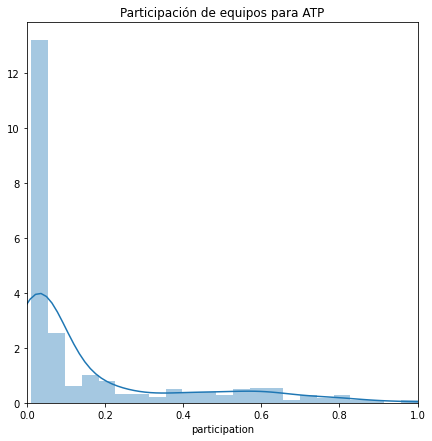
\includegraphics[scale=0.5]{img/reales/atp-part.png}
        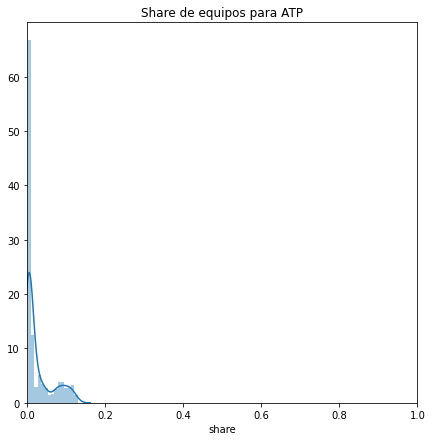
\includegraphics[scale=0.5]{img/reales/atp-share.png}
        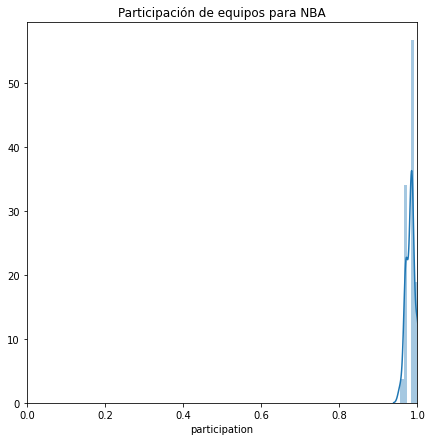
\includegraphics[scale=0.5]{img/reales/nba-part.png}
        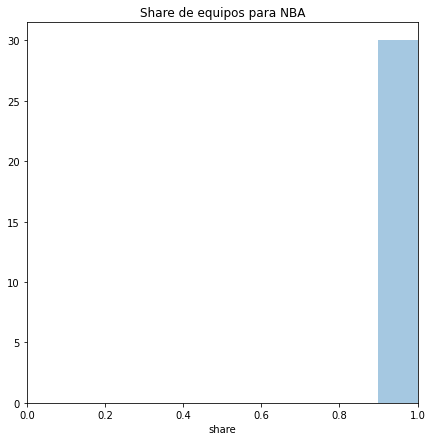
\includegraphics[scale=0.5]{img/reales/nba-share.png}
        \caption{Participacion y share de ATP vs NBA}
        \label{real-part-share}
    \end{center}
\end{figure}

Como se puede ver en la figura \ref{real-part-share},
\begin{itemize}
    \item NBA sería ideal para WP, ya que al ser round robin, todos jugaron contra todos (el share es 1), y casi todos jugaron la misma cantidad de juegos (la participación de casi todos es 1). Debería dar muy similar los ratings resultantes entre WP y CMM.
    \item ATP es lo contrario, no juegan todos contra todos, y tampoco juegan la misma cantidad de juegos. Debería dar diferente entre WP y CMM.
\end{itemize}

\subsection{Justeza de CMM}

Nos interesa estudiar si CMM es un método \textit{justo}, es decir, si los partidos entre dos jugadores podrían afectar a un tercero que no tiene relación con ellos. Además, la \textit{afectación} se puede ver con respecto a dos aspectos: el \textbf{rating} (numero que el método le asigna a cada equipo) y \textbf{ranking} (ordenando todos los equipos por su rating, en que posición queda).

\subsubsection{Rating}

Suponiendo que juegan los equipos $d$ con $e$, ¿Podría el resultado de su partido afectar a un tercero, $a$? Nuestra hipótesis es que depende de cual sea la definición de \textit{tercero} empleada.
Por como se conforma la matriz de colley, el rating de un equipo depende del rating de sus oponentes. Entonces, si $a$ no jugó contra $d$ ni $e$, en principio su rating no debería verse afectado, pero si había jugado por ejemplo contra $b$, que \textbf{sí} había jugado contra $c$ y este contra $d$, el rating de $c$ y $d$ se vería afectado, y luego el de $a$ también.

Podemos ver los dos casos posibles con el siguiente esquema, que representa a cada equipo como un nodo en un grafo, y existe una conexión entre ellos si jugaron al menos un partido:

\begin{figure}[H]
    \begin{subfigure}{.5\textwidth}
        \centering
        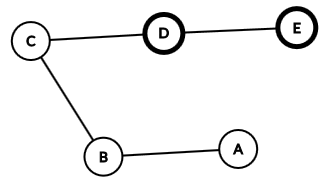
\includegraphics[scale=0.5]{img/grafos/CaminoConectado.png}
        \caption{Camino conectado}
        \label{camino-conectado}
    \end{subfigure}
    \begin{subfigure}{.5\textwidth}
        \centering
        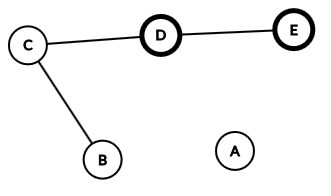
\includegraphics[scale=0.5]{img/grafos/CaminoNoConectado.png}
        \caption{Camino desconectado}
        \label{camino-desconectado}
    \end{subfigure}
    \caption{Posibles relaciones entre equipos}
\end{figure}

\begin{itemize}
    \item En \ref{camino-conectado}, podemos ver que, A no jugó contra D y E, pero sin embargo existe un camino que une a A con D y E, debido a que hay una cadena de relaciones entre equipos que jugaron entre si. En este caso, el rating se vería afectado por este juego. 
    \item En cambio, en \ref{camino-desconectado}, el equipo A no tiene relación, ni siquiera indirecta con ellos, ya que no existe un camino que los conecte. Luego, su rating no se verá afectado.
\end{itemize}
\subsubsection{Ranking}

El ranking \textbf{siempre} debería poder cambiar, ya que aunque el rating no se vea afectado, siempre que se vea afectado el de otra persona, podría cambiar el orden de la tabla de posiciones, lo cual cambiaría su ranking.

\subsection{Análisis de estrategias}

Una pregunta que uno podría hacerse mientras analiza el método CMM, es si existe una estrategia que permita obtener el \textit{mayor ranking posible}, con la \textit{menor} cantidad de victorias.
Para poder determinar estas estrategias, tomamos los resultados de una competencia, elegimos un equipo, y aplicamos una de varias heurísticas para así minimizar la cantidad de victorias. Y para hacerlo lo más realista posible, establecemos tres restricciones sobre qué es posible modificar

\begin{itemize}
    \item Solo se pueden cambiar los resultados de los partidos en los que participó el equipo seleccionado.
    \item Solo se pueden \textit{perder} partidos que previamente habían sido ganados, y no ganar partidos que habían sido perdidos. Esto es porque nos parece razonable la noción de que uno podría decidir hacer \textit{forfeit} de un juego, pero nunca podría asegurar una victoria.
    \item El jugador seleccionado conoce las habilidades reales del resto.
\end{itemize}

\subsubsection{Simulador de partidos}

Para poder probar estas heurísticas o estrategias en un ambiente lo más controlado posible, haremos uso de un \textit{simulador de partidos} en vez de usar datos reales. Este nos permite, a grandes rasgos, controlar la \textbf{habilidad} de cada equipo y como se distribuye, y el \textbf{schedule} que siguen los partidos. Luego, para cada partido entre dos equipos, la probabilidad de ganar de cada uno es proporcional a su habilidad.

\begin{itemize}
    \item La habilidad será distribuida de forma \textit{lineal}, es decir, sea $N$ el máximo poder y $T$ la cantidad de equipos, el poder $p_i$ de cada equipo queda determinado por la siguiente ecuación

    \begin{align*}
        p_i = i * \frac{N}{T}
    \end{align*}
    
    \item El \textit{schedule} a seguir será \textit{round robin}. Es decir, juegan todos contra todos.
\end{itemize}

\subsubsection{Heurísticas}
A continuación describimos las diferentes heurísticas que proponemos para lograr el objetivo propuesto: maximizar el ranking, minimizando la cantidad de victorias.

\paragraph{Naive}
Las heurísticas \textbf{lose\_better} y \textbf{lose\_worse} son muy simples, perder todos los partidos contra los que tengan mayor y menor habilidad, respectivamente. Dada su simpleza, esperamos que sean las peores.

Dado el funcionamiento del método CMM, pesan más los partidos ganados contra mejores oponentes. De esto se deriva la última estrategia \textit{naive}, \textbf{win\_one}. Esta se encarga de perder \textit{todos} los partidos menos uno, el que ganó contra el equipo con mayor rating.

\paragraph{Hill Climber}
La heurística \textbf{hill climber} toma el estado actual de los datos de la competencia, selecciona al azar un juego en el que esté involucrado y haya ganado, lo modifica para perder y recalcula el ranking de colley. Con esto obtiene su nuevo rating, y toma una decisión dependiendo si es mejor o peor que el anterior. Si es igual o mejor, acepta el nuevo estado ya que minimizo sus ganadas sin empeorar su ranking.

Este proceso se repite durante varias iteraciones con el objetivo de poder minimizar lo mas posible sus ganadas. Esta forma de estrategia es también \textit{naive} en cierto sentido, ya que selecciona juegos al azar, y acepta un nuevo estado solo porque se acerco un poco a su objetivo. 

Tiene el problema de que puede quedarse atrapado en un mínimo local, cuando tal vez era mejor tomar otra decisión la cual a la larga lograría minimizar aun mas las partidas ganadas.

\paragraph{min\_cmm}

Quisiéramos alguna manera de perder la mayor cantidad de juegos posibles sin perjudicar nuestra posición en el ranking. De esta manera, la estrategia se reduce a averiguar qué oponente es más conveniente para cederle una victoria. Luego, la estrategia consiste en perder contra estos oponentes hasta que otra derrota más implique un descenso en la tabla de posiciones. Si analizamos definición del 'rating' de un jugador en base al sistema asociado a la matriz de Colley, podremos observar que este está determinado, más allá de las victorias y derrotas del propio jugador, por los ratings de sus oponentes, y la cantidad de juegos que el jugador tiene en común.

\[r_i = \frac{1}{2+n_i}\Big(1 + \frac{n_w - n_l}{2} + r_{1}n_{i1} + \ldots + r_{n}n_{in}\Big)\]

Lo que esto significa es que, en un formato donde juegan todos contra todos, en términos de diferencias absolutas del rating de un equipo, nos es indiferente contra quién perdemos. Perder contra cualquier oponente nos significa la misma caída del rating que contra cualquier otro, y además esta derrota significa el mismo aumento del rating para todos los otros equipos. Con esto, podemos responder cuál es el oponente más conveniente para cederle una victoria: el último en la tabla de posiciones. La justificación es bastante simple, queremos que el oponente que vaya a incremente su número de victorias ($n_w$), sea el que está a mayor distancia de alcanzar nuestra posición. Lo interesante de esta estrategia es que, al ceder una victoria, el estado inicial de la competencia cambia, y no necesariamente se mantiene quién esta último en la tabla de posiciones. Este concepto es parte fundamental de esta heurística y nos permite minimizar la cantidad de victorias necesarias para mantener el ranking.

En cada iteración, la heurística,
\begin{enumerate}
    \item Calcula los ratings actuales.
    \item Modifica los juegos para perder contra aquel oponente que está último en la tabla de los ratings.
    \item Calcula los ratings nuevamente
    \item Si su posición en el ranking bajó, entonces volvemos uno atrás y finalizamos. Sino, repetimos el proceso hasta que suceda.
\end{enumerate}

\section{Resultados y discusión}

\subsection{Error CMM}

Estos son los resultados de medir el error entre nuestra implementación del \textbf{Colley Matrix Method},y nuestro sujeto de comparación, la solución del sistema asociado a la matriz de Colley, computado por la biblioteca \texttt{numpy.linalg}. También medimos el grado de error incluído en los ratings provistos por la cátedra.

\begin{figure}[H]
    \begin{center}
        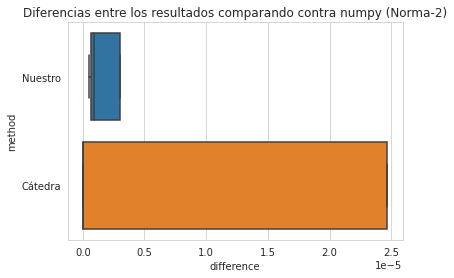
\includegraphics[scale=0.75]{img/prec/n2.png}
        \caption{Error medido por la norma euclídea}
        \label{prec-norma2}
    \end{center}
\end{figure}

\begin{figure}[H]
    \begin{subfigure}{.5\textwidth}
        \centering
        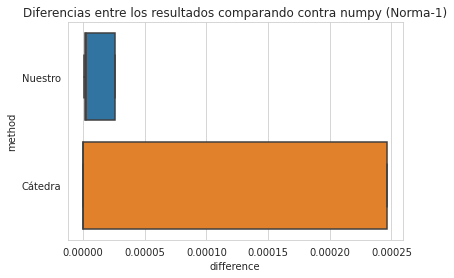
\includegraphics[scale=0.5]{img/prec/n1.png}
        \caption{Error medido por la norma-1}
        \label{prec-norma1}
    \end{subfigure}
    \begin{subfigure}{.5\textwidth}
        \centering
        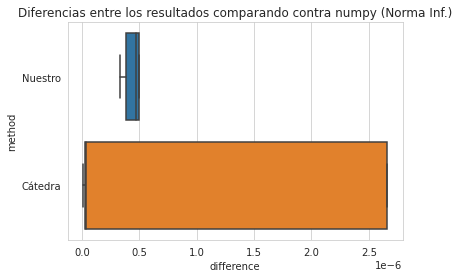
\includegraphics[scale=0.5]{img/prec/index.png}
        \caption{Error medido por la norma infinito}
        \label{prec-normainf}
    \end{subfigure}
\end{figure}

Como se puede ver en la figura \ref{prec-norma2}, en todos los casos, utilizando todas las normas vectoriales, nuestros resultados resultan más precisos que los provistos por la cátedra. Lo que resulta interesante es que, dentro de todas las normas utilizadas, la que menor varianza tiene es la norma infinito,. Esto tiene sentido dado que si muchos de los componentes tienen algún error proveniente de usar aritmética finita, estos no se suman entre si, cosa que sucede al calcular la distancia utilizando otras normas vectoriales.

\subsection{Comparativa entre métodos}

Los resultados de correr los rankings son los siguientes

\begin{figure}[H]
    \begin{subfigure}{.5\textwidth}
        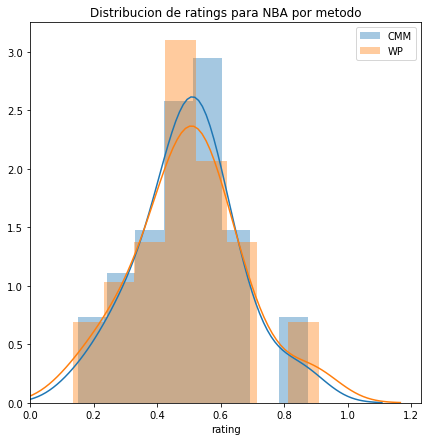
\includegraphics[scale=0.5]{img/reales/nba-ranking.png}
        \caption{Rankings para NBA}
        \label{rankings-nba}
    \end{subfigure}
    \begin{subfigure}{.5\textwidth}
        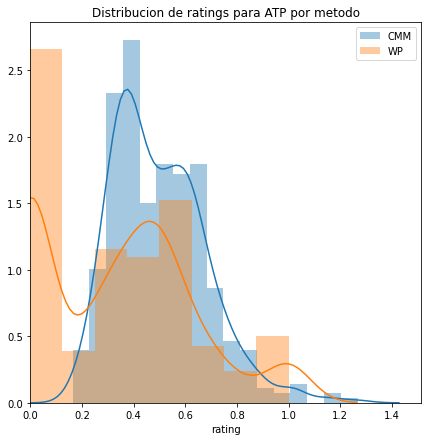
\includegraphics[scale=0.5]{img/reales/atp-ranking.png}
        \caption{Rankings para ATP}
        \label{rankings-atp}
    \end{subfigure}
    \caption{Comparativas de rankings}
\end{figure}

Como se puede ver en la figura \ref{rankings-nba}, el ranking coincide para NBA tanto para WP como CMM, pero este este no es el caso de ATP como ilustra \ref{rankings-atp}, donde varían significativamente los rankings resultantes de ambos métodos. Además, como en ATP muchos no jugaron tantos partidos (ya que su participación era baja), su ranking oscila al rededor del inicial de cada método, 0 para WP y 0.5 para CMM.

\subsection{Justeza de CMM}

El experimento que hicimos fue tomar los datos utilizados en \textit{Govan et al}\footnote{http://carlmeyer.com/pdfFiles/SASGF08RankingPaper.pdf}, que daban como ranking inicial,

\begin{figure}[H]
    \begin{center}
        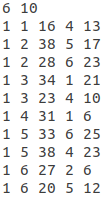
\includegraphics[scale=0.6]{img/justo/govan-orig.png}
        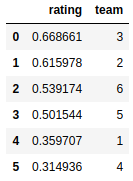
\includegraphics[scale=0.75]{img/justo/govan-rating-original.png}
        \caption{Data y rankings resultantes con los datos originales de Govan}
        \label{govan-orig}
    \end{center}
\end{figure}

Y modificarlos para que tengan dos nuevos equipos que hayan jugado entre sí pero contra nadie más, el 7 y 8 (el ultimo juego)

\begin{figure}[H]
    \begin{center}
        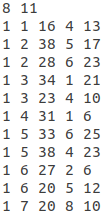
\includegraphics[scale=0.75]{img/justo/govan-changed.png}
        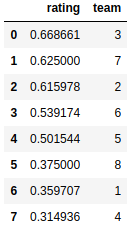
\includegraphics[scale=0.75]{img/justo/govan-rating-changed.png}
        \caption{Data y rankings resultantes con los datos modificados de Govan}
        \label{govan-changed}
    \end{center}
\end{figure}

Como se puede ver en la figura \ref{govan-changed}, los nuevos equipos, 7 y 8, tienen ranking 2 y 6 respectivamente. Para ver si estos cambian después de juegos de terceros, agregamos a los datos partidos entre 5 y 6, que no están relacionados ni indirectamente con 7 y 8.

\begin{figure}[H]
    \begin{center}
        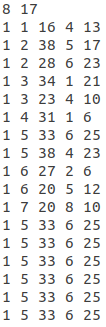
\includegraphics[scale=0.75]{img/justo/govan-new.png}
        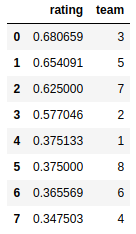
\includegraphics[scale=0.75]{img/justo/govan-rating-new.png}
        \caption{Data y rankings resultantes con los datos nuevos de Govan}
        \label{govan-new}
    \end{center}
\end{figure}

Como se puede ver en la figura \ref{govan-new}, a pesar de que los ratings de 7 y 8 permanecen exactamente iguales, el ranking de 7 se ve afectado, pasando de 2do a 3ro, ya que cambiaron los ratings del resto de los equipos, lo cual confirma nuestras hipótesis.

\subsection{Análisis de estrategias}

La simulación a realizar tiene 10 equipos, y el elegido para aplicar las heurísticas es el numero 8, (el tercero mejor) ya que tendrá muchas partidas ganadas en las cuales hacer \textit{forfeit}. Para comparar las heurísticas entre sí, tendremos en cuenta dos métricas: \textit{ranking resultante} y \textit{wins}. De esta forma, podremos observar cual es la que minimiza las wins maximizando el ranking.

Comenzamos por determinar una \textit{seed}, para que luego la simulación con cada heurística sea reproducible y obtengamos los mismos resultados. Primero lo simulamos sin aplicar ninguna heurística, y luego sobre el conjunto de partidos resultantes aplicamos cada una. Esto lo iteramos 50 veces, y los resultados son los siguientes:

\begin{figure}[H]
    \begin{center}
        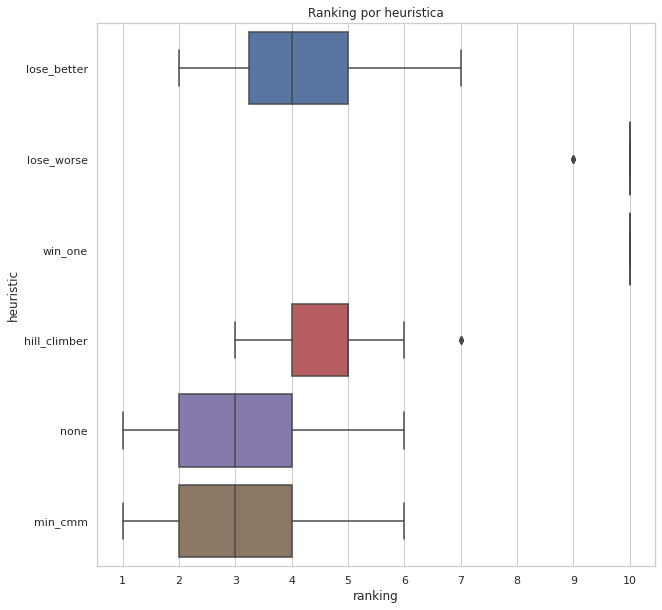
\includegraphics[scale=0.45]{img/heur/ranking-inicial.png}
        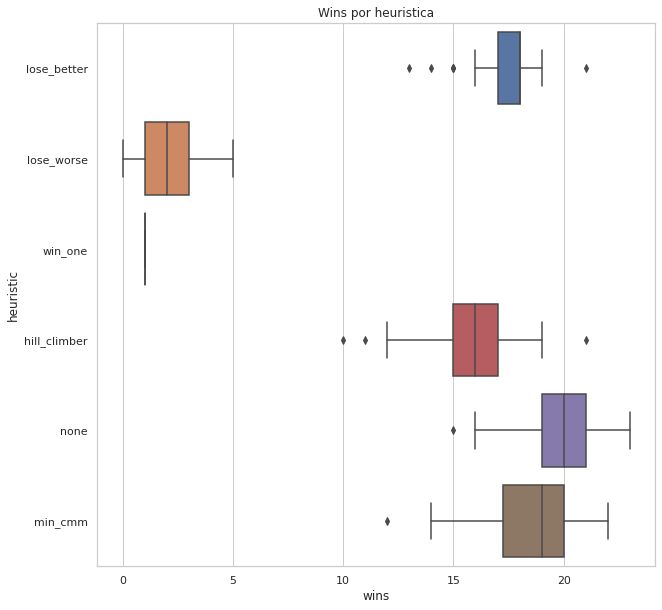
\includegraphics[scale=0.45]{img/heur/wins-inicial.png}
        \caption{Ranking y wins obtenido por cada heurística luego de haber modificado los juegos}
        \label{heur-initial}
    \end{center}
\end{figure}

Como se puede ver en la figura \ref{heur-initial},

\begin{itemize}
    \item \textbf{none} es el resultado de no aplicar ninguna heurística, un resultado de \textit{control} para comparar con el resto.
    \item \textbf{lose\_worse} es el peor, ya que al ser el equipo numero 8, como las habilidades son lineales, casi todos son peores que él, entonces pierde casi todos los juegos, lo cual afecta demasiado a su ranking previo a los cambios.
    \item \textbf{win\_one} muestra que al parecer, no basta con ganar solo una para tener un ranking competente, ya que sale consistentemente último.
    \item \textbf{lose\_better} resultó ser eficaz para ser tan simple. Las wins son consistentemente menores que sin heurísticas, pero el ranking disminuyó bastante.
    \item \textbf{hill\_climber} es parecido al anterior, con la diferencia de que \textit{siempre} pierde ranking, pero es el que menos victorias tiene hasta el momento.
    \item \textbf{min\_cmm} es el mejor y se comporta como era esperado. El ranking es siempre idéntico, y las wins son consistentemente menores, tal como buscábamos.
\end{itemize}

Luego de haber concluido que \textbf{min_cmm} era el mejor, decidimos buscar otra forma de visualizar el comportamiento del mismo. Para ello, consideramos la evolución del rating de cada equipo fecha por fecha.

\begin{figure}[H]
    \begin{center}
        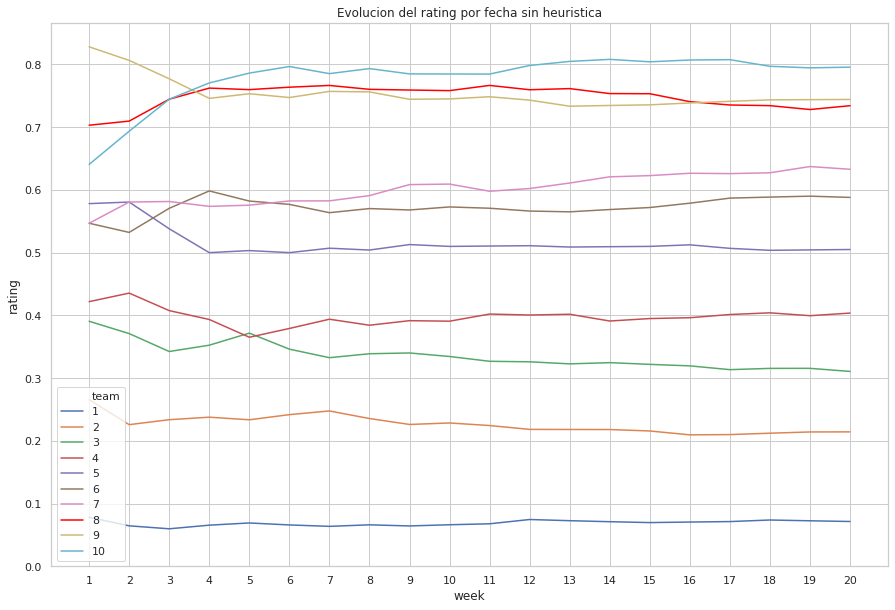
\includegraphics[scale=0.45]{img/heur/evol-sin-heuristica.png}
        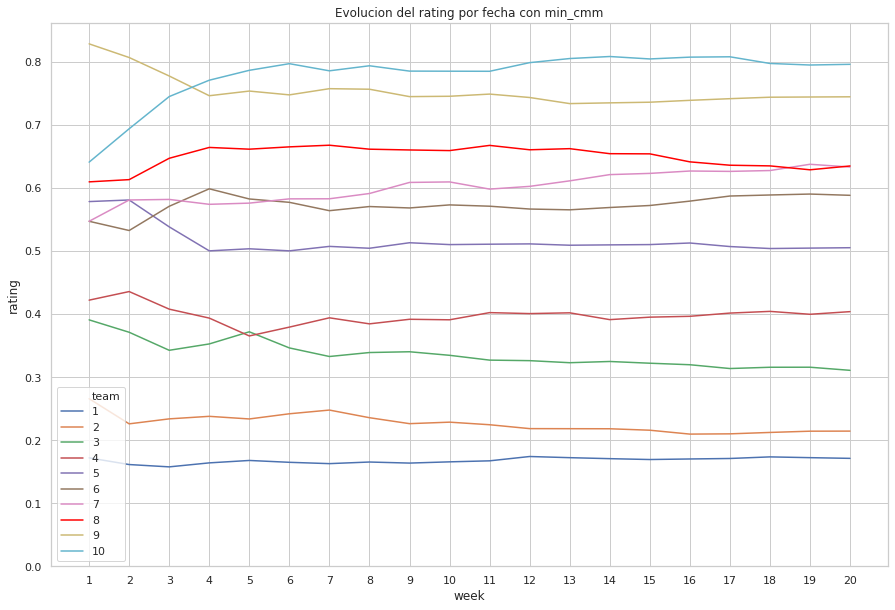
\includegraphics[scale=0.45]{img/heur/evol-min-cmm.png}
        \caption{Rating semana a semana sin heurística y aplicando min cmm}
        \label{heur-evol}
    \end{center}
\end{figure}

Como se puede ver en la figura \ref{heur-evol}, el equipo elegido (el 8), se deshace de la diferencia de rating innecesaria entre el y el anterior (el 7), hasta \textit{justo} antes de perder un rank. Además, los ratings del último equipo suben, ya que ahora le gana al equipo elegido muchos mas partidos.

Además, el rating de cada equipo se ve correlacionado con su habilidad real. Lo que ilustra que el método CMM produce resultados que reflejan la habilidad real de los equipos.

\subsubsection{Tolerancia de perdida de ranking}

Hay casos en donde no es de interés mantener el ranking exacto, como por ejemplo en las selecciones de un mundial de fútbol, donde lo importante es quedar entre los primeros. En esos casos, se podría \textit{tolerar} perder algunos ranks, y así se tener aún menos victorias.

Para modelar esto, introducimos una nueva clase de heurísticas: \textit{min cmm con \textbf{tolerancia}}. Estas \textit{tolera} perder N ranks, en pos de seguir minimizando sus victorias. Con esta consideración, la implementación inicial de min cmm tendría \textit{tolerancia 0}, por ejemplo.

Esto produce que pierda muchos mas partidos, pero sin embargo no llegaba a bajar todos los ranks que le permitía su tolerancia. Esto se debe a que se queda sin partidos que perder contra el último, porque se rinde en todos los posibles. Por esta razón, le agregamos la capacidad de, en el caso de no poder perder mas contra el ultimo, empezar a perder contra el ante último, luego el antepenúltimo, y así. Los resultados fueron los siguientes

\begin{figure}[H]
    \begin{center}
        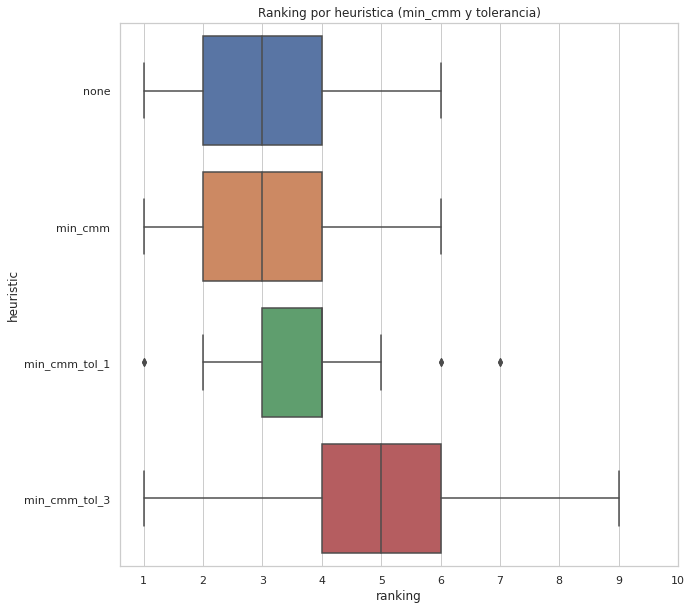
\includegraphics[scale=0.45]{img/heur/ranking-min-cmm.png}
        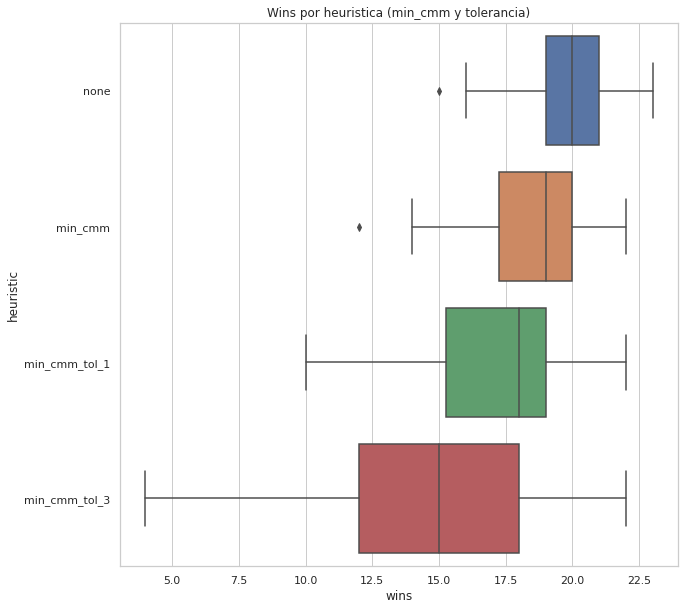
\includegraphics[scale=0.45]{img/heur/wins-min-cmm.png}
        \caption{Ranking y wins obtenido por cada heurística de la clase min cmm con tolerancia. Donde $min\_cmm\_tol\_i$ tolera perder $i$ ranks}
        \label{heur-min-cmm-tol}
    \end{center}
\end{figure}

En la figura \ref{heur-min-cmm-tol} se puede ver que estas nuevas heurísticas se comportan como es esperado, perdiendo la cantidad de ranks que toleran y en consecuencia, las wins bajan sustancialmente. También podemos ver su comportamiento analizando fecha a fecha

\begin{figure}[H]
    \begin{center}
        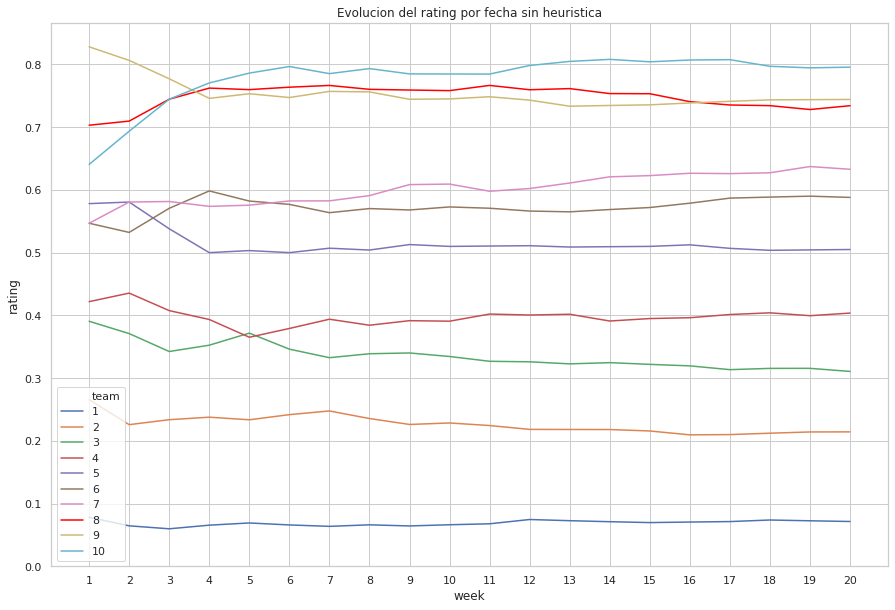
\includegraphics[scale=0.25]{img/heur/evol-sin-heuristica.png}
        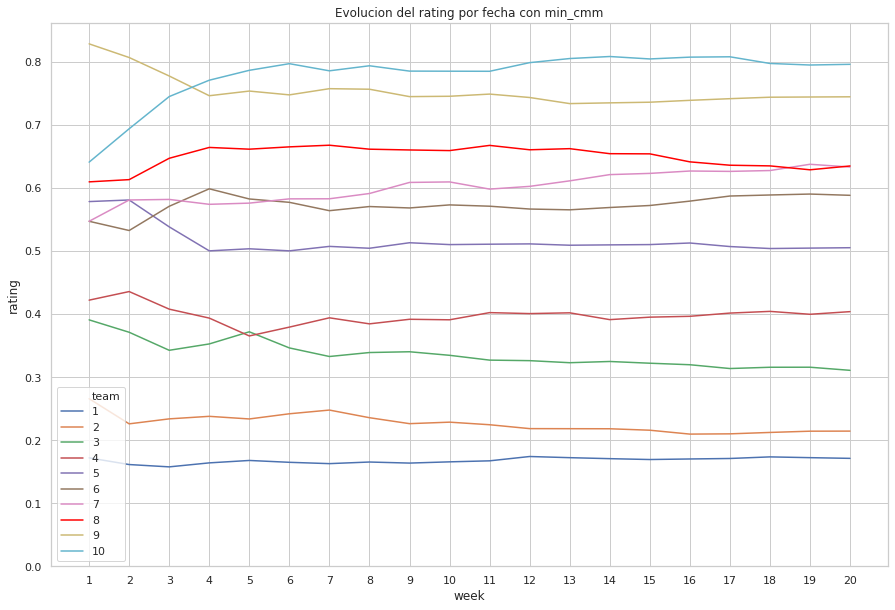
\includegraphics[scale=0.25]{img/heur/evol-min-cmm.png}
        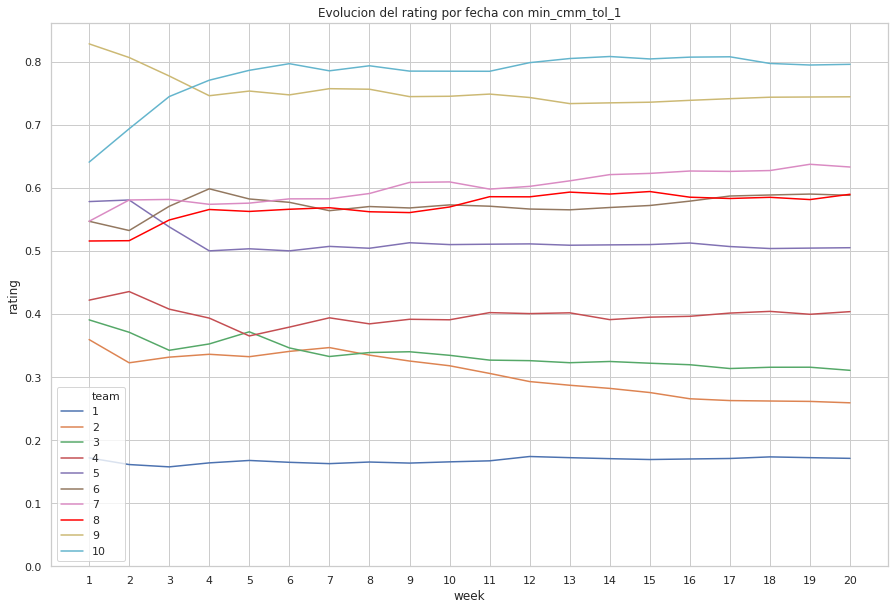
\includegraphics[scale=0.25]{img/heur/evol-min-cmm-tol-1.png}
        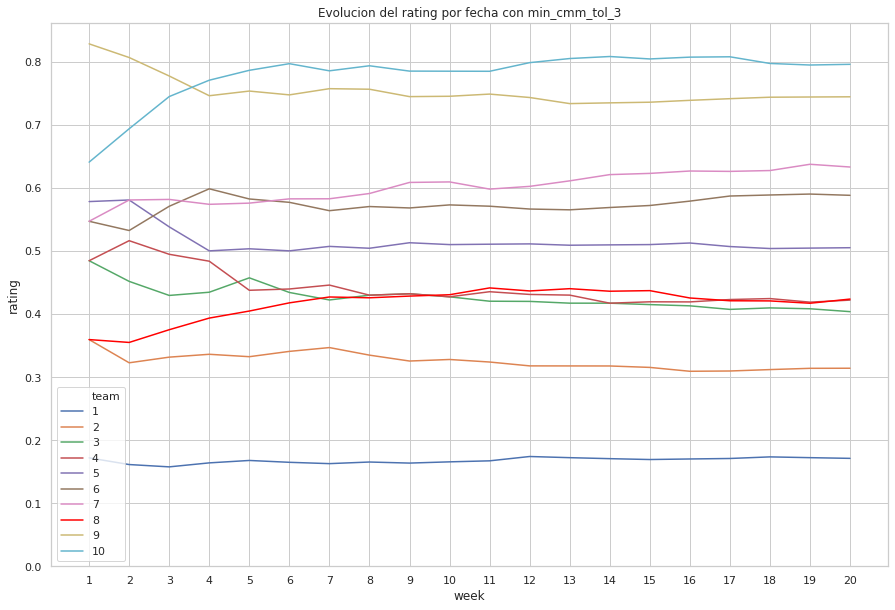
\includegraphics[scale=0.25]{img/heur/evol-min-cmm-tol-3.png}
        \caption{Rating fecha a fecha sin heuristica y aplicando min cmm con niveles variables de tolerancia}
        \label{heur-evol-cmm}
    \end{center}
\end{figure}

En la figura \ref{heur-evol-cmm} Se puede ver como, claramente, al final del torneo el equipo elegido se queda con el rating que le permita mantener \textit{justo} la pérdida de ranking tolerado. También es posible notar que, como pierde contra más jugadores, una mayor proporción de los ratings se ve afectada, ya que mas equipos ganan partidos además del ultimo. Esto ultimo es interesante porque, aunque muchos ratings de equipos se vean afectados, sus rankings finales no se ven afectados, demostrando como CMM mantiene una relación entre los equipos y sus ratings.

%==========MATRIZ GENERICA=========
%\begin{equation*}
%A_{m,n} = 
%\begin{pmatrix}
%a_{1,1} & a_{1,2} & \cdots & a_{1,n} \\
%a_{2,1} & a_{2,2} & \cdots & a_{2,n} \\
%\vdots  & \vdots  & \ddots & \vdots  \\
%a_{m,1} & a_{m,2} & \cdots & a_{m,n} 
%\end{pmatrix}
%\end{equation*}
%==================================
\section{Conclusión}

Como también concluye Colley en su paper original\footnote{https://www.colleyrankings.com/matrate.pdf}, WP no es un buen método para confeccionar rankings, dado su mal funcionamiento para ciertos formatos de competencias, i.e diferentes a \textit{round-robin}. Sin embargo, CMM parece producir rankings que reflejan de cierta forma la realidad, ya que para los jugadores simulados, su rating estaba relacionado a su habilidad real.

Al margen de la correctitud del método CMM, consideramos que es un método \textit{justo}. Ya que los ratings de un equipo son afectados por los juegos de otros solo cuando estaban de cierta forma relacionados entre sí.

En cuanto a las heurísticas, si bien concluimos que la mejor es \textit{min\_cmm}, esto es solo en el caso en el que formato de la competencia sea \emph{round-robin}. Sino, podría mejorarse la elección del oponente, ya que se debe tener en cuenta la cantidad de partidos que este tuvo contra el resto, y si es baja, tal vez el impacto en el rating de los otros jugadores no sea tanto. 

Además, este y el resto de las estrategias empleadas buscan, dado un rank, mantenerlo (o incluso, empeorarlo) minimizando las victorias necesarias. Pero lo que \textbf{no} buscan, y podría ser un punto interesante para futuras investigaciones, es mejorar ese ranking inicial. Para ello, tal vez habría que cambiar el enfoque utilizado, y en vez de modificar una lista de partidos ya dada, tomar decisiones sobre la marcha, basándose en la información disponible en el momento.

\end{document}

\end{figure}
